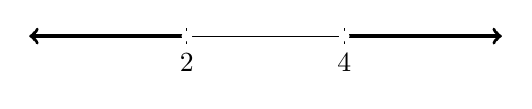
\begin{tikzpicture}
	\draw[<->] (0,0) -- (6,0);
	\draw (2,0.1) -- + (0,-0.2) node[below] {$2$};
	\draw (4,0.1) -- + (0,-0.2) node[below] {$4$};
	\draw[<-, very thick, \colorone] (0,0) -- (2,0);
	\draw[->, very thick, \colorone] (4,0) -- (6,0);
	\fill[white, draw=\colorone] (2,0) circle (0.6mm);
	\fill[white,draw=\colorone] (4,0) circle (0.6mm);
\end{tikzpicture}
%\captionof{figure}{Graphically and numerically approximating $\lim_{x\to 3} \frac{x^2-x-6}{6x^2-19x+3}$ in Example \ref{ex_limit1}.}
%\caption{Graphically and numerically approximating $\lim_{x\to 3} \frac{x^2-x-6}{6x^2-19x+3}$ in Example \ref{ex_limit1}.}
%\label{fig:limit1}
